\documentclass{beamer}

\usepackage[utf8]{inputenc}
\usepackage{graphicx}
\usepackage{tikz-cd}
\usepackage{bm}
\usepackage{amsmath,amssymb,amsthm}
\usepackage{pgfplots}
\usepackage{xcolor}
\usepackage[shortlabels]{enumitem}
\usepackage[mathscr]{euscript}
\pgfplotsset{compat = newest}
\usepackage{float}
\usepackage{microtype}
\usepackage[mode=text]{siunitx}
\usepackage{longtable}

% Special definitions
\newcommand{\Sha}{\rotatebox[origin=c]{180}{$\Pi\kern-0.347em\Pi$}}


\title{Ordinal Pattern Features: Statistical Properties and Their Applications in Time Series Clustering}
\author[Rasika Dilhani]{{Rasika Dilhani}\\{\small Supervisors: Alejandro C.\ Frery and Andrea A.\ Rey}}
\institute[VUW]{Victoria University of Wellington}
\date{16 July 2025}

\usetheme{Madrid}

%\titlegraphic{\includegraphics[width=2cm]{logopolito}\hspace*{4.75cm}~%
   %
\includegraphics[width=2cm]{VUW_Standard_Landscape_BLACK.eps}
%}
\titlegraphic{
\includegraphics[width=4cm]{VUW_Standard_Landscape_BLACK.eps}
}
% Change base colour beamer@blendedblue (originally RGB: 0.2,0.2,0.7)
\definecolor{VUWgreen}{RGB}{0,71,48}
\colorlet{beamer@blendedblue}{VUWgreen}


\begin{document}

\maketitle
%outline
\begin{frame}{Outline}
    \tableofcontents
\end{frame}

%--------------------%
\section{Introduction}
%--------------------%
%--------------------%
%\subsection{Approaches to time series analysis}
%--------------------%

\begin{frame}{What is a Time Series?}
	\begin{itemize}
		\item A \textbf{time series} is a sequence of observations $x_t$, each indexed by time $t$ (discrete or continuous).
		\item Each $x_t$ is a realization of a random variable $X_t$.
		\item \textbf{Examples:}
		\begin{itemize}
			\item Finance: stock prices, exchange rates
			\item Biology: heart rate, population growth
			\item Geoscience: weather, humidity
		\end{itemize}
		\end{itemize}
		\begin{figure}[hbt]
			\centering
			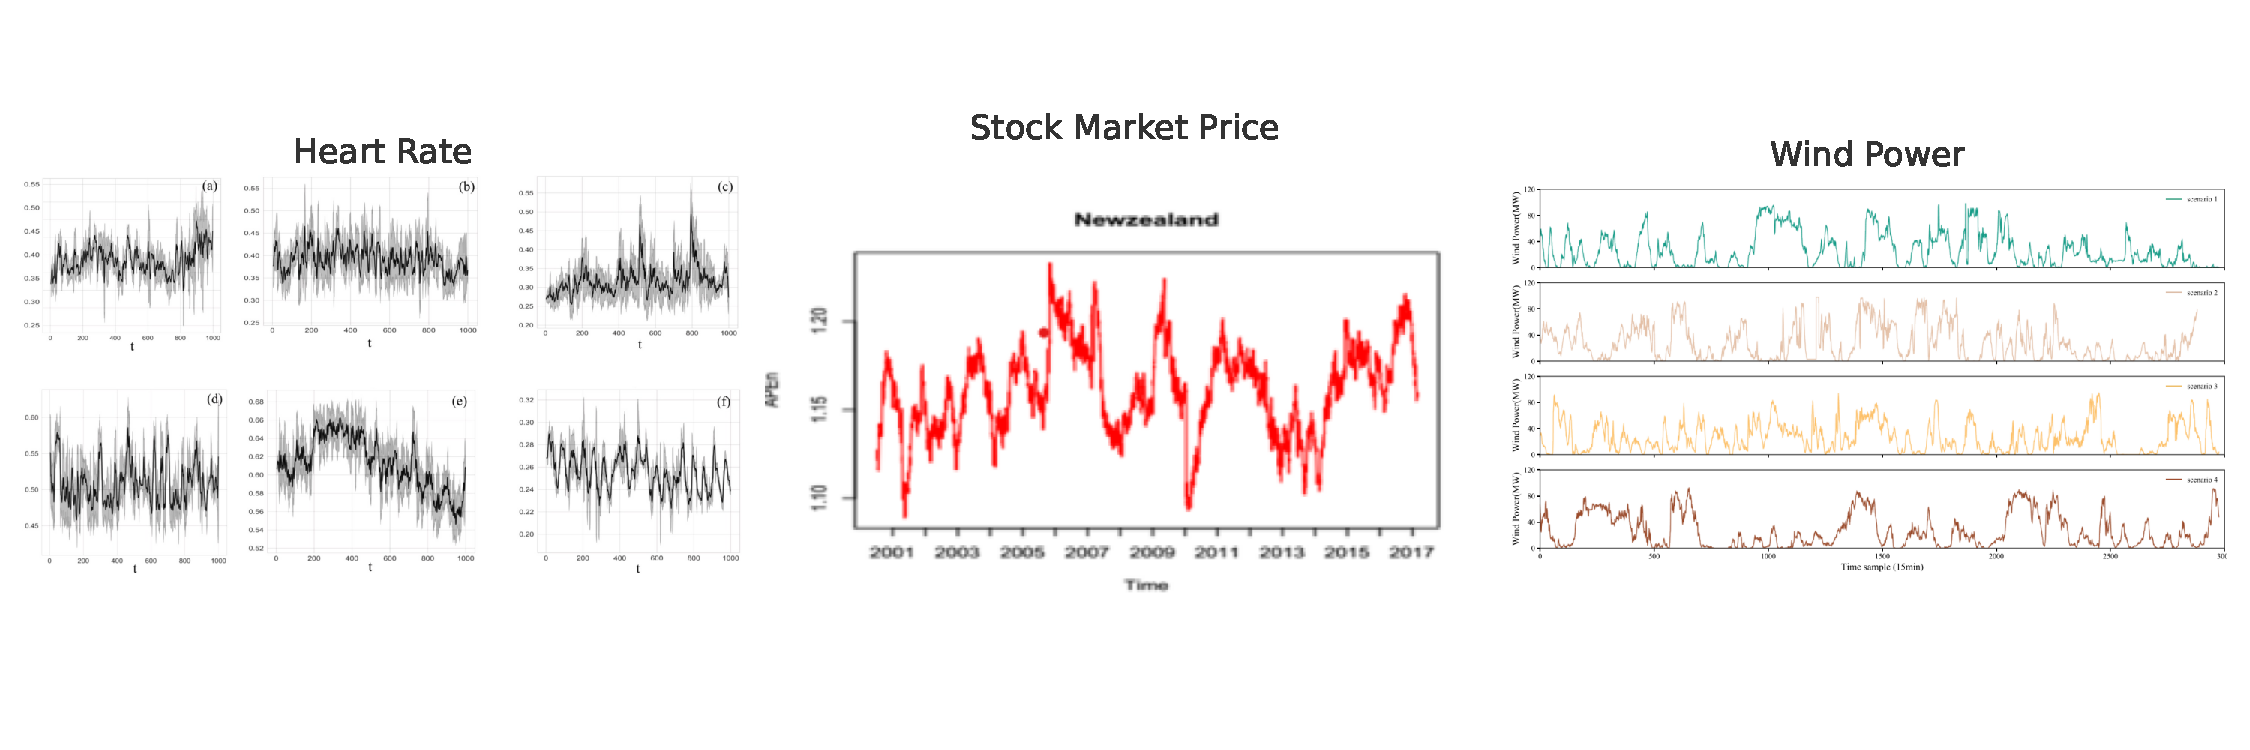
\includegraphics[width=0.6\textwidth]{time series plots}
			\caption{Examples for Biology, Finance, and Geoscience: sources from Silva et.al., Patra et.al. and Meng et.al.~\cite{Silva2023,Patra2022,Meng2023}}
			\label{fig:timeseries}
		\end{figure}	
%%% ACF Illustrate with one time series from each example (on the same slide)
\end{frame}

\begin{frame}{Why Analyze Time Series?}
	\begin{itemize}
		\item Understand underlying system dynamics.
		\item Forecast future values.
		\item Detect anomalies or pattern changes. %%% ACF You haven't defined stationarity yet; better say "changes"
	\end{itemize}
\end{frame}


%---------------------------%
%\subsection{The Bandt-Pompe Approach: Successes and Limitations}
%---------------------------%

\begin{frame}{The Bandt-Pompe Approach: Motivation and Context}
	\begin{itemize}
		\item \textbf{Time series} contain valuable insights about the underlying system that generates the data.
		\item Traditional analysis uses two main approaches: time-domain and frequency-domain.
		%\begin{itemize}
		%	\item \textbf{Time-domain methods:} Analyze relationships between current and past values.
		%	\item \textbf{Transformed-domain methods:} Use spectral expansions (e.g., Fourier, wavelets).
		%\end{itemize}
		\item Many classical statistical methods make assumptions (large sample sizes, normality) that are often violated in real data, leading to unreliable results.
	\end{itemize}
\end{frame}

\begin{frame}{The Bandt-Pompe Approach: Successes and Limitations}
	\begin{itemize}
		\item \alert{Ordinal patterns:} Capture the order relations among consecutive values in a time series.
		\item \alert{Bandt \& Pompe (2002) \cite{PhysRevLett.88.174102}:} Transform time series into ordinal patterns, build a histogram of patterns, and compute Shannon entropy aka Permutation Entropy.
		\item \textbf{Advantages:}
		\begin{itemize}
			\item Non-parametric (no distribution assumptions)
			\item Robust to outliers and monotonic transformations
			\item Captures temporal structure
		\end{itemize}
		\item \textbf{Limitations:}
		\begin{itemize}
			\item Sensitive to equal (tied) values
			\item Choice of embedding parameters affects results
			\item May not capture long-range dependencies
		\end{itemize}
	\end{itemize}
\end{frame}

%%% ACF A new slide illustrating the symbolisation

\begin{frame}{Complexity}
	While Permutation Entropy is a powerful tool for quantifying disorder, it does not fully capture the complexity of dynamical systems.
	
	Entropy measures randomness, but cannot distinguish between purely random and structured (complex) behaviors.
	
	To address this, López-Ruiz et al.~\cite{lopez1995statistical} introduced the concept of \alert{disequilibrium}, quantifying the deviation of a probability distribution from a uniform (maximally disordered) state.
	
	Using the disequilibrium defined by Lamberti et al. \cite{lamberti2004intensive}, another descriptor, statistical complexity is used to analyze time series.  
\end{frame}

\begin{frame}{The Entropy-Complexity Plane: Mapping Dynamics}
	The \alert{entropy-complexity plane} is a two-dimensional representation where time series are mapped according to their entropy ($H$) and statistical complexity ($C$).
	
	Both metrics are derived from ordinal pattern distributions, obtained by mapping a time series into histograms.
	% of $D!$ bins.
	
	This framework enables the distinction between different types of dynamics based on their location in the plane.
\end{frame}

\begin{frame}{Statistical Properties of Entropy, Complexity, and Related Features}
	Based on the literature review, determining the exact distribution of \alert{features} from ordinal patterns is challenging; therefore, researchers have extensively investigated this distribution and its related statistical properties.
%	First simplification
	\begin{itemize}
		\item \textbf{Empirical distributions:} Constructed directly from observed data, these distributions reflect the actual frequencies of patterns or outcomes.
		\item \textbf{Asymptotic distributions:} Two types of asymptotic distributions are discussed: the first assumes that patterns are independent and identically distributed (Multinomial Model), while the second considers patterns that are dependent.
		\item \textbf{Other features:} Beyond entropy and complexity, related statistical measures such as Tsallis entropy, Rényi entropy, and Fisher information have also been studied for their asymptotic properties.
	\end{itemize}
\end{frame}

%%% ACF The previous slide presents the BP (2002)
%%% The next, your proposal
%%% But your proposal also uses the complexity
%%% You need an intermediate slide (or a couple of slides) that situates the audience in the state-of-the-art:
%%% The HxC manifold and what we know about the statistical properties of these (and other) features
%%% Only then, you present the general and specific objetives

%---------------------------%
%\subsection{General and specific objectives of research work}
%---------------------------%

\begin{frame}{General and specific objectives of research work}
	\begin{itemize}
		\item \textbf{General Objective: To answer the following question}
		\begin{itemize}
			\item How can confidence intervals for generalized entropy measures (Shannon, Tsallis, Rényi, Fisher information measure) and their associated complexity metrics be used to improve the 
			%%% ACF I would avoid "robustness" here because you are referring to the robustness of conclusions, but the OPs are robust to transformations in a different way
			reliability and discriminative power of time series clustering techniques?
		\end{itemize}
	\end{itemize}		
		
The literature review shows that confidence intervals have not been used to assess the reliability of entropy and complexity measures in time series analysis; therefore, we are motivated to study this issue.
%%% ACF Where have they been used?
\end{frame}

\begin{frame}{General and specific objectives of research work (cont..)}
\begin{itemize}
	\item \textbf{Main Objectives:}
	\begin{itemize}
		%%% ACF Add, in your own words, review the literature and verify if the claims hold when using confidence regions for the features
		\item Define a data base of time series for clustering, i.e., finding similar time series. 
		\item Extract all the features we know from their Bandt \& Pompe symbolization (Shannon, Tsallis and Renyi entropies, Fisher information measure, complexities, and the available confidence intervals).
		\item Use those features for time series clustering.
	\end{itemize} 
\end{itemize}	

\end{frame}


%---------------------------%
\section{Literature Review}
%---------------------------%
\begin{frame}
	\begin{center}
		\alert{Literature Review}
	\end{center}
\end{frame}

%---------------------------%
%\subsection{which statistical results do we know about features from ordinal patterns?}
%---------------------------%

\begin{frame}{Known statistical results about features from ordinal patterns}
%%% ACF These slides are central to your work. You must know what each reference does
	\begin{itemize}
		\item \textbf{Normal (Gaussian) distribution:}
		%%% ACF Does the normal law appear only under independence or only without independence or in both cases?
		\begin{itemize}
			\item Describes the asymptotic behavior of entropy and complexity estimators derived from ordinal patterns~\cite{Chagas2022, Rey2023, Rey2023a, Rey2024, Rey2025}.
			%%% ACF Did Chagas et al use the normal distribution?
		\end{itemize}
		\item \textbf{Chi-squared ($\chi^2$) distribution:}
		\begin{itemize}
			\item Arises in tests for randomness, independence, and serial dependence in ordinal patterns~\cite{Rey2023, Rey2024, Rey2025, YamashitaRiosDeSousa2022, Shternshis2025}.
		\end{itemize}
	\end{itemize}
\end{frame}

\begin{frame}{Known statistical results about features from ordinal patterns (cont.)}
	\begin{itemize}
		\item \textbf{Empirical (permutation) distributions:}
		\begin{itemize}
			\item Used in non-parametric independence and randomness tests by shuffling data to generate the null distribution~\cite{MatillaGarcia2008, AshtariNezhad2019}.
			\item Used in white noise tests by repeatedly shuffling the time series to estimate the null distribution of the test statistic~\cite{Chagas2022a}.
		\end{itemize}
		\item \textbf{Alpha-stable distributions:}
		\begin{itemize}
			\item Applied for feature extraction in heavy-tailed or non-Gaussian environments, such as fault diagnosis~\cite{Chouri2014}.
		\end{itemize}
	\end{itemize}
\end{frame}

\begin{frame}{Known statistical results about features from ordinal patterns (cont.)}
	\begin{itemize}
		\item \textbf{Markov transition probabilities:}
		\begin{itemize}
			\item Used to model the dynamics of ordinal patterns as Markov processes~\cite{Sakellariou2019}.
		\end{itemize}
		\item \textbf{Belief functions and evidence theory:}
		\begin{itemize}
			\item Provide a framework for quantifying uncertainty using Deng entropy and mass assignments, extending beyond classical probability~\cite{Xie2025}.
		\end{itemize}
	\end{itemize}
\end{frame}


%---------------------------%
\section{Methodology}
%---------------------------%

\begin{frame}
	\begin{center}
		\alert{Methodology}
	\end{center}
\end{frame}

%---------------------%
%\subsection{Ordinal Patterns}
%---------------------%

\begin{frame}{From Time Series to Ordinal Patterns: An Example}
%%% ACF Make this graphical
	\begin{itemize}
		\item \textbf{Given:} Mean monthly humidity in Wellington,
		\begin{itemize}
			\item January, February, March, April, May, June, etc...
			\item 77.3, 81.0, 82.4, 81.7, 83.6, 85.6, etc... 
		\end{itemize}
	\end{itemize}
\begin{figure}[hbt]
	\centering
	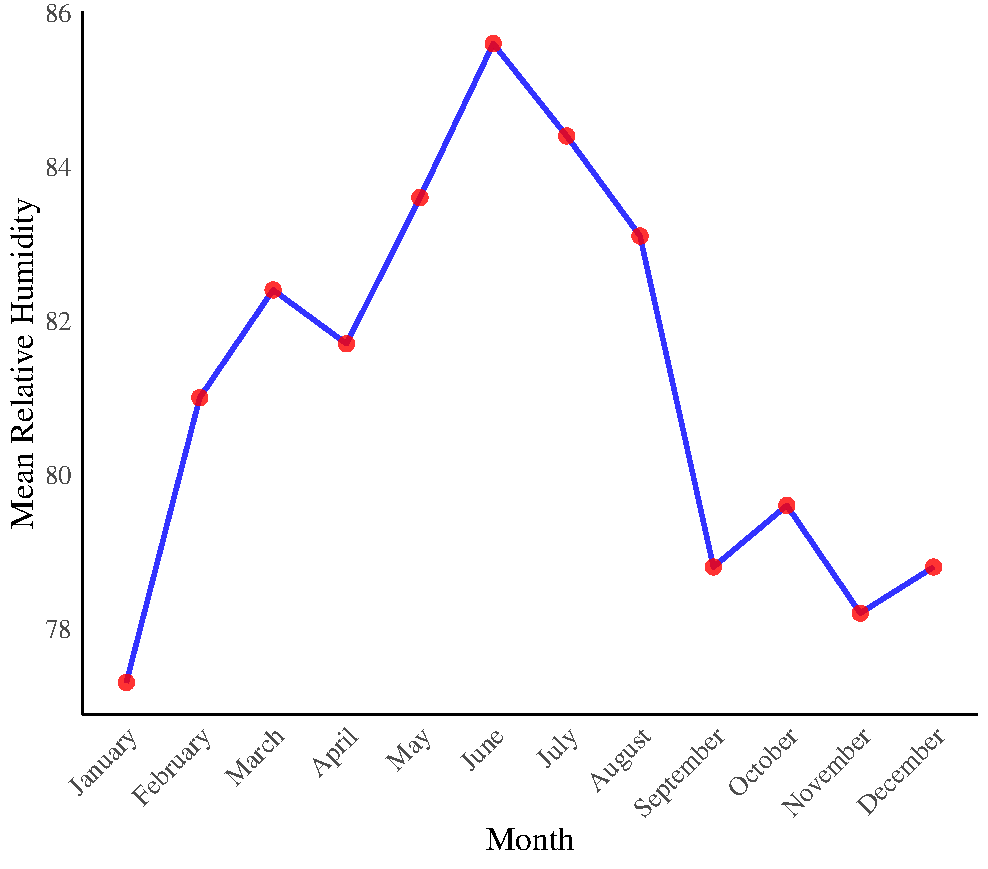
\includegraphics[width=0.6\textwidth]{humidity graph}
	\caption{Mean Monthly humidity in Wellington}
	\label{fig:humidity}
\end{figure}	
	
\end{frame}

\begin{frame}{Transforming to Ordinal Patterns}
	For $D=3$, where $D$ is called as \alert{embedding dimension}.
	
	The first window (77.3, 81.0, 82.4) $\rightarrow$ Pattern: (1,2,3) $\rightarrow \pi^1$.
	
	Next window (81.0, 82.4, 81.7) $\rightarrow$ Pattern: (1,3,2) $\rightarrow \pi^2$.
	
	Continue for all overlapping windows.
	
	%%% ACF Check
	We have $n+D-1$ overlapping windows, where $n$ represents the series length. 
\end{frame}

%---------------------%
%\subsection{Histogram}
%---------------------%

\begin{frame}{Histogram of Ordinal Patterns}
	Count the frequency of each ordinal pattern.\\
	For $D=3$, there are $3!=6$ possible patterns: (1,2,3), (1,3,2), (2,1,3), (2,3,1), (3,1,2), (3,2,1).\\
	The histogram shows the proportion of each pattern in the time series.
\end{frame}

\begin{frame}{Visualizing the Histogram}
	The histogram provides a visual summary of the distribution of ordinal patterns.\\
	Peaks indicate frequent 
	%%% ACF "common" or "frequent"?
	patterns; valleys indicate rare patterns.\\
	This distribution is the basis for computing the entropy and the complexity 
	%%% ACF Only the entropy? Remember: you work in the HxC manifold!
	calculation.
		\begin{center}
		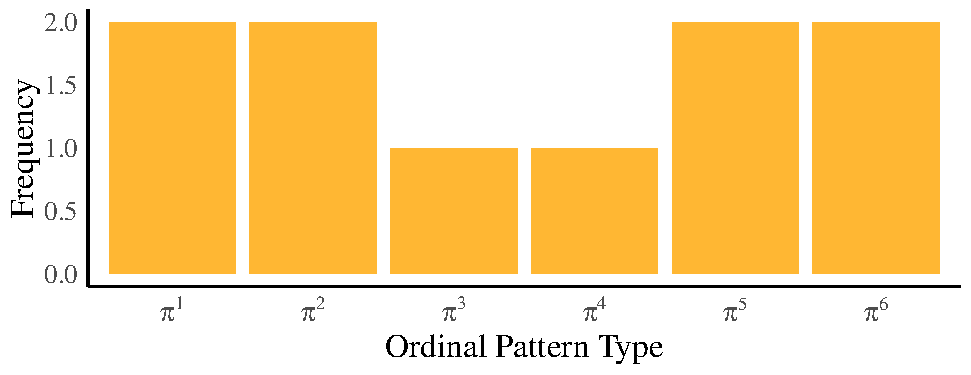
\includegraphics[width=0.7\textwidth]{frequency histogram}
	\end{center}
\end{frame}

%---------------------%
%\subsection{Entropy}
%---------------------%

\begin{frame}{Shannon Entropy and Permutation Entropy}

%%% ACF reformulate. It sounds as if you were presenting two totally different things

	Entropy measures, such as \alert{Shannon entropy} (which quantifies the uncertainty in a probability distribution) and \alert{Permutation entropy} (which measures the complexity of the order structure in time series using ordinal patterns), are used to quantify the degree of randomness or disorder in data. 
	\begin{block}{Definition:}
		\[
		H(\mathbf{p}) = -\dfrac{1}{\log k} \sum_{i=1}^{k} p(\pi^i) \log p(\pi^i),
		\]
		where $k=D!$ and $p(\pi^i)$ is the proportion of pattern $\pi^i$.
	\end{block}
	High entropy: patterns are equally likely (randomness).\\
	Low entropy: some patterns dominate (regularity/structure).
\end{frame}

%---------------------%
%\subsection{Complexity}
%---------------------%

%\begin{frame}{Complexity}
%	While Permutation entropy is a powerful tool for quantifying disorder, it does not fully capture the complexity of dynamical systems.\\
%	Entropy measures randomness, but cannot distinguish between purely random and structured (complex) behaviors.\\
%	To address this, López-Ruiz et al.~\cite{lopez1995statistical} introduced the concept of \textbf{disequilibrium} $Q$, quantifying the deviation of a probability distribution $\mathbf{p}$ from a uniform (maximally disordered) state.
%\end{frame}

\begin{frame}{Measuring Disequilibrium: Jensen-Shannon Distance to calculate complexity}
	
%%% ACF Read this slide outloud; does it sound good?
	López-Ruiz et al.~\cite{lopez1995statistical} used the \alert{Euclidean distance}; Lamberti et al.~\cite{lamberti2004intensive} proposed the \alert{Jensen-Shannon distance} for ordinal pattern distributions.
	\begin{block}{Definition:Disequilibrium}
		%%% ACF Missing punctuation after equations
		For a histogram $\mathbf{p}$ and uniform distribution $\mathbf{u}=(1/k, \ldots, 1/k)$ ($k=D!$):
		\[
		Q'(\mathbf{p},\mathbf{u}) = \sum_{\ell=1}^k \Big( p_\ell \log\frac{p_\ell}{u_\ell} + u_\ell \log\frac{u_\ell}{p_\ell} \Big).
		\]
		Normalized disequilibrium:
		\[
		Q = \frac{Q'}{\max(Q')},
		\]
		where $\max(Q')$ is the maximum possible value of $Q'$.
		%%% ACF Alredy cited. Do not cite the same work many times. 
	\end{block}
\end{frame}

\begin{frame}{Statistical Complexity: Combining Entropy and Disequilibrium}
	\begin{itemize}
		\item Lamberti et al.~\cite{lamberti2004intensive} defined \alert{statistical complexity} $C$ as:
		\begin{block}{Definition:Complexity}
			\[
			C = H Q
			\]
			where $H$ is normalized entropy and $Q$ is normalized disequilibrium.
		\end{block}
		\item $C$ is also normalized, ranging from 0 (minimal complexity) to 1 (maximal complexity).
		\item This measure captures both randomness and structure, providing a richer description of time series dynamics than entropy alone.
	\end{itemize}
\end{frame}


%---------------------%
%\subsection{The Entropy-Complexity manifold, its boundaries and "areas" according to the literature}
%---------------------%
%\begin{frame}{The Entropy-Complexity Plane: Mapping Dynamics}%
%	The \alert{entropy-complexity plane} is a two-dimensional representation where time series are mapped according to their entropy ($H$) and statistical complexity ($C$).
	
%	 Both metrics are derived from ordinal pattern distributions, obtained by mapping a time series into histograms of $D!$ bins.
	 
%	This framework enables the distinction between different types of dynamics based on their location in the plane.
%\end{frame}


\begin{frame}{Boundaries and Structure in the Plane}
	\begin{itemize}
		\item Martin et al.~\cite{Martin2006} derived expressions for the boundaries of the entropy-complexity plane using geometric arguments.
		\item The \alert{lower boundary} is a smooth curve; the \alert{upper boundary} consists of $D!-1$ segments, becoming smoother as $D \to \infty$.
		\item These boundaries provide a structured approach to analyzing the spatial behavior of specific systems or models.
		\item \textbf{Example:} The entropy-complexity plane for embedding dimensions 3, 4, 5, and 6 is shown below.
		\begin{center}
			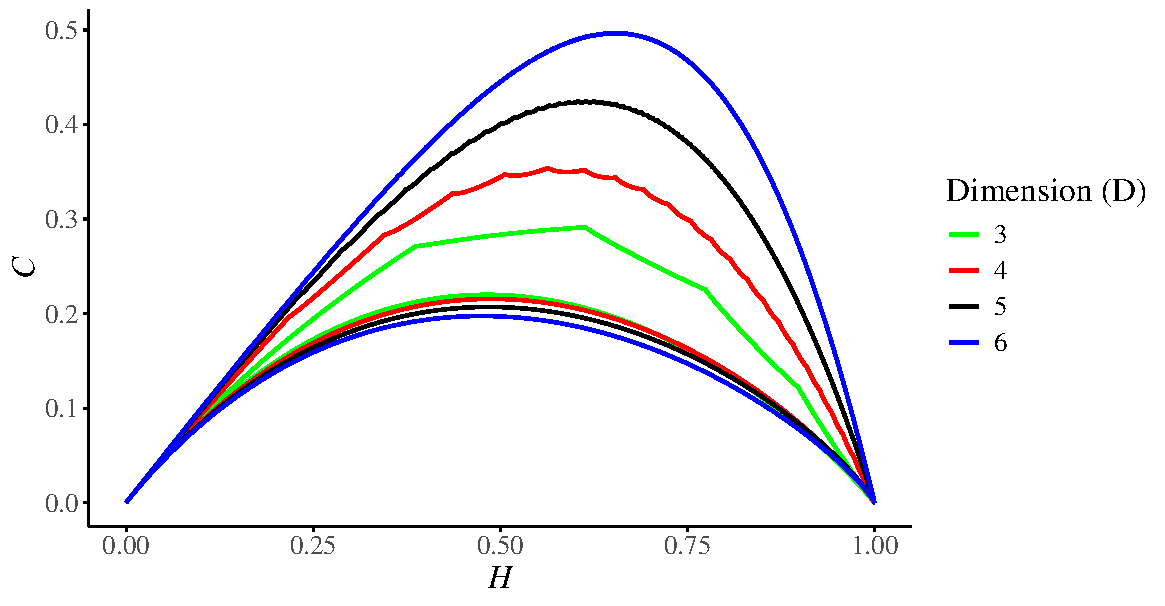
\includegraphics[width=0.6\textwidth]{complexity plane}
		\end{center}
	\end{itemize}
\end{frame}

\begin{frame}{Ten time series and their points in the $H \times C$ plane for embedding dimension 6 according to our application}
	%The $H \times C$ plane, with bounds corresponding to embedding dimension 6, shows the mapped points for each time series according to our application.
	\begin{center}
		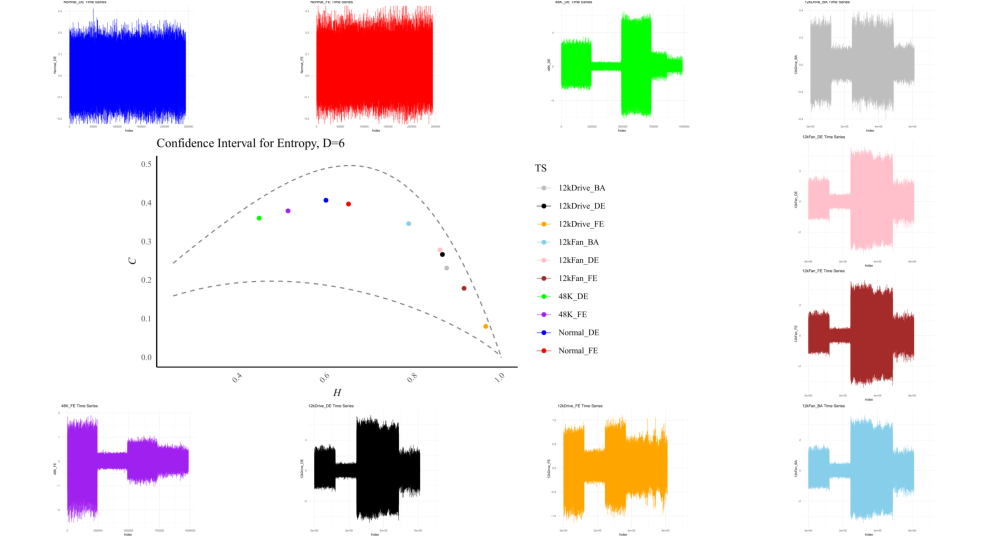
\includegraphics[width=0.8\textwidth]{combined plot}
	\end{center}
	
\end{frame}

%%% ACF Make your own version of Fig. 4 from Chagas et al. (2022) with representative examples

%---------------------%
%\subsection{Asymptotic distribution of the Entropy}
%---------------------%

\begin{frame}{Asymptotic distribution of the Entropy and complexity}
	%%% ACF Only entropy? We discussed this! Revise everything.
	Three types of Asymptotic distribution of entropy and complexity are discussed.
	\begin{itemize}
		\item Empirical Approach
		\item Incorporating with independence pattern: Multinomial model 
		\item Incorporating dependence among patterns
	\end{itemize}
\end{frame}

%%% ACF Asymptotic and Empirical do not go together
\begin{frame}{Asymptotic Distribution of Entropy and complexity: Empirical Approach}
What is an \alert{Empirical Distribution}?
	\begin{itemize}
		\item It is a probability distribution constructed directly from observed data, without assuming any theoretical model.
		\item It is built by counting how often each outcome appears in the data and dividing by the total number of observations.
		\item \textbf{Key features:}
		\begin{itemize}
			\item \textbf{Data-driven:} Reflects the actual frequencies observed in the sample.
			\item \textbf{Non-parametric:} Makes no assumptions about the underlying distribution.
			\item \textbf{Flexible:} Useful for any data type, especially when the true distribution is unknown.
		\end{itemize}
	%	\item \textbf{Example:} In ordinal pattern analysis, the empirical distribution describes the observed frequencies of each pattern in the time series, forming the basis for entropy and complexity calculations.~\cite{Chagas2022a}
	\end{itemize}
\end{frame}


\begin{frame}{Multinomial Model for Ordinal Patterns}
	\begin{itemize}
		%%% ACF \bm p and \boldmath p for the same. We had talked about this. Revise everything
		\item Imagine $n$ independent trials, each resulting in one of $k$ mutually exclusive outcomes $\pi^1, \pi^2, \ldots, \pi^k$ with probabilities $\mathbf{p} = (p_1, \ldots, p_k)$, where $\sum_{\ell=1}^{k} p_\ell = 1$.
		\item The random vector $\mathbf{N} = (N_1, \ldots, N_k)$ counts the number of occurrences of each outcome in $n$ trials, with $\sum_{\ell=1}^{k} N_\ell = n$.
		\item The joint distribution is:
		\[
		\Pr(\mathbf{N} = \mathbf{n}) = n! \prod_{\ell=1}^{k} \frac{p_\ell^{n_\ell}}{n_\ell!}
		\]
		\item This is denoted as $\mathbf{N} \sim \text{Mult}(n, \mathbf{p})$~\cite{Rey2023}.
	\end{itemize}
\end{frame}


\begin{frame}{Asymptotic Distribution of Entropy and complexity under the Multinomial Law}
	\begin{itemize}
		\item The estimated Shannon entropy is:
		\begin{block}{Definition: Estimated Shannon Entropy}
			\[
			H(\widehat{\mathbf{p}}) = -\sum_{\ell=1}^k \hat{p}_\ell \log \hat{p}_\ell, \quad \text{where } \hat{p}_\ell = \frac{N_\ell}{n}
			\]
		\end{block}
	
		\item As the sample size $n \rightarrow \infty$, $H(\widehat{\mathbf{p}})$ converges to a normal distribution, even for dependent processes:
		\[
		\sqrt{n}(H(\widehat{\mathbf{p}}) - H(\mathbf{p})) \xrightarrow{d} \mathcal{N}(0, \sigma^2)
		\]
		\item This provides a theoretical foundation for using entropy and complexity as statistical tools when probabilities are estimated from finite samples~\cite{Rey2023}.
	\end{itemize}
\end{frame}


\begin{frame}{Asymptotic Distribution of Entropy and complexity under the Multinomial Law (cont..)}
	After calculating the estimated entropy, we can calculate the estimated disequilibrium $Q(\widehat{\mathbf{p}})$ 
	
	\begin{block}{Estimated complexity under the Multinomial model}
		\[	C[\widehat{\bm{p}}]=H[\widehat{\bm{p}}]Q[\widehat{\bm{p}}].\]
	\end{block}
\end{frame}

\begin{frame}{Asymptotic Distribution of Entropy and complexity: Incorporating dependence among patterns}
	\begin{itemize}
		\item Given a real-valued time series $\mathbf{x} = \{x_1, x_2, \ldots, x_{n+D-1}\}$, we extract ordinal patterns by transforming overlapping subsequences of embedding dimension $D$ into symbols: $\mathbf{\pi} = (\pi_1, \pi_2, \ldots, \pi_n)$.
		\item The number of possible patterns is $k = D!$.
		\item Due to the overlapping windows, the resulting ordinal patterns are \textbf{dependent}.
		\item For each $i = 1, 2, \ldots, k$, let $p_i$ be the probability of observing the pattern $\pi_i$, and define the probability vector $\mathbf{p} = (p_1, p_2, \ldots, p_k)$.
		\item The diagonal matrix of probabilities is $\mathbf{D_p} = \text{Diag}(p_1, p_2, \ldots, p_k)$.
	\end{itemize}
\end{frame}

\begin{frame}{Transition Probabilities and Dependence Structure}
	\begin{itemize}
		\item The transition probability of moving from state $\pi_i$ at time $t$ to state $\pi_j$ at time $t+r$ (for $r = 1, 2, \ldots, D-1$) is denoted $p^{(r)}_{ij}$.
		\item All such transition probabilities can be collected in the matrix $\mathbf{Q}^{(r)}$ with entries $p^{(r)}_{ij}$.
		\item These matrices capture the dependence structure among ordinal patterns due to overlapping windows.
		\item Even though patterns are dependent, this structure can be explicitly modeled and incorporated into statistical analysis.
	\end{itemize}
\end{frame}

\begin{frame}{Asymptotic Distribution for Entropy and Complexity}
	\begin{itemize}
		\item When the sample size $n$ is sufficiently large, the \textbf{asymptotic distribution} of the Shannon entropy can be used, even in the presence of dependence among patterns~\cite{Rey2023a}.
		\item The asymptotic variance of the entropy estimator accounts for the dependence structure and is given by:
	\begin{block}{Definition: Asymptotic Variance}
		\[
			\begin{split}
				\sigma^2_{\mathbf{p}} = & \sum_{i=1}^{k}(\ln p_i + 1)^2 
				\left[ p_i - (2D - 1)p_i^2 + 2\sum_{r=1}^{D-1} \mathbf{Q}^{(r)}_{ii} \right] \\
				& - 2 \sum_{i=1}^{k-1} \sum_{j=i+1}^{k} (\ln p_i + 1)(\ln p_j + 1) \\
				& \quad \times \left[ (2D - 1)p_i p_j - \sum_{r=1}^{D-1} \left( \mathbf{Q}^{(r)}_{ij} + \mathbf{Q}^{(r)}_{ji} \right) \right].
			\end{split}
			\]
	\end{block}
	\end{itemize}
\end{frame}

\begin{frame}{Asymptotic Distribution for Entropy and Complexity (cont..)}
	Thus for practical purpose, given $n$ is sufficiently large, we can assume that $H(\widehat{\mathbf{p}})$ has a normal distribution with mean equal to $H(\widehat{\mathbf{p}})$ and variance equal to $\sigma^2_{\widehat{\mathbf{p}}}/n$.
	
	In addition to that, for $\alpha\in(0,1)$ and $n$ sufficiently large, the $(1-\alpha)\SI{100}{\percent}$ confidence interval of $H(\widehat{\mathbf{p}})$ is given by, 
	\begin{block}{Definition: Confidence Interval}
		\[
		H(\widehat{\mathbf{p}})\pm \dfrac{Z_{\alpha/2}\sigma_{\widehat{\mathbf{p}}}}{\sqrt{n}},
		\label{eq:ConfidenceInterval}
		\]
		where $Z_{\alpha/2}$ is the $\alpha/2$-quantile of a standard normal random variable.
	\end{block} 
\end{frame}


%---------------------%
%\subsection{Other types of entropy measures}
%---------------------%

\begin{frame}{Other types of Entropy: Tsallis Entropy}
	\begin{itemize}
		\item \textbf{Tsallis entropy} is a generalization of Shannon entropy, introducing a parameter $q$ to control sensitivity to probability distribution.
		\item It is useful for analyzing systems with long-range interactions.
		\item The Tsallis entropy of order $q$ is defined as:
		\begin{block}{Tsallis Entropy}
			\[
			H_{T}^{q}(\widehat{\mathbf{p}}) = \sum_{\ell=1}^{k} \frac{\widehat{p_\ell} - \widehat{p_\ell}^q}{q-1}
			\]
			where $q \in \mathbb{R} \setminus \{1\}$
		\end{block}
		\item For $q \to 1$, Tsallis entropy converges to Shannon entropy.
	\end{itemize}
\end{frame}

\begin{frame}{Other types of Entropy: Rényi Entropy}
	%%% ACF Does the Rényi entropy follow asymptotically a normal distribuiton?
	\begin{itemize}
		\item \textbf{Rényi entropy} is another generalization of Shannon entropy, parameterized by $q$.
		\item It emphasizes different aspects of the distribution depending on the value of $q$.
		\item The Rényi entropy of order $q$ is defined as:
		\begin{block}{Definition:Rényi entropy }
			\[
			H_{R}^{q}(\widehat{\mathbf{p}}) = \frac{1}{1-q} \log \left( \sum_{\ell=1}^{k} \widehat{p_\ell}^q \right)
			\]
			where $q \in \mathbb{R}^+ \setminus \{1\}$
		\end{block}
		\item For $q \to 1$, Rényi entropy also converges to Shannon entropy.
	\end{itemize}
\end{frame}

\begin{frame}{Other types of Entropy: Fisher Information}
	%discrete case
	\begin{itemize}
		\item \textbf{Fisher information} measures the sensitivity of a probability distribution to small changes, capturing local structure and regularity.
		\item For discrete distributions, it is approximated by differences between consecutive probabilities:
		\begin{block}{Definition: Fisher Information}
			\[
			H_F(\widehat{\mathbf{p}}) = F_0 \sum_{\ell=1}^{k-1} \left( \sqrt{{\widehat{p}_{\ell+1}}} - \sqrt{\widehat{p_\ell}} \right)^2
			\]
			where the normalization coefficient $F_0 = 4$
		\end{block}
		\item Fisher information is more sensitive to small changes and perturbations than entropy.
	\end{itemize}
\end{frame}



%---------------------%
%\subsection{The StatOrdHxC package; its contents and limitations}
%---------------------%

\begin{frame}{The StatOrdPattHxC Package: Contents}
	\begin{itemize}
		\item \textbf{StatOrdPattHxC} is a package for statistical analysis of time series using ordinal patterns.
		\item \textbf{Key features and functions:}
		\begin{itemize}
			\item Computes normalized Shannon, Rényi, and Tsallis entropies, as well as Fisher information and statistical complexity.
			\item Calculates ordinal pattern probabilities (\texttt{OPprob}) and sequences (\texttt{OPseq}) for a given embedding dimension.
			\item Provides tools for hypothesis testing between time series (\texttt{entropicTest}, \texttt{pval}), including asymptotic variance calculations for entropy and complexity (\texttt{asymptoticVarHShannonMultinomial}, \texttt{sigma2q}, \texttt{meanC}, \texttt{varC}).
			\item Determines boundaries for the entropy-complexity ($H \times C$) manifold (\texttt{LinfLsup}) and computes moving averages (\texttt{mov.av}).
		\end{itemize}
		\item The package supports robust, non-parametric inference for time series features under the multinomial model, making it suitable for a wide range of scientific and engineering applications.
	\end{itemize}
\end{frame}

\begin{frame}{StatOrdPattHxC: Limitations and Practical Considerations}
	\begin{itemize}
		\item \textbf{Computational limitations:}
		\begin{itemize}
			\item The number of possible ordinal patterns grows factorially with the embedding dimension ($D!$), leading to rapid increases in computational complexity.
			%%% ACF Are the features the problem? NO
			\item For large datasets or embedding dimensions greater than 3, calculations (such as entropy, complexity, and hypothesis testing) can become extremely time-consuming—potentially taking more than a week for a single analysis.
		\end{itemize}
		\item \textbf{Practical advice:}
		\begin{itemize}
			\item Choose embedding dimensions carefully, balancing the need for detailed pattern analysis with available computational resources.
			\item For very large time series or high $D$, consider parallel computing or dimensionality reduction techniques.
		\end{itemize}
		\item Despite these challenges, StatOrdPattHxC remains a powerful tool for extracting and statistically validating features from time series using ordinal pattern analysis.
	\end{itemize}
\end{frame}

\begin{frame}
	\begin{center}
		\alert{Results}
	\end{center}
\end{frame}

%---------------------%
\section{Results}
%---------------------%
\begin{frame}{Case Study: Bearing Fault Detection Data}
	\begin{itemize}
		\item \textbf{Data Source:} Bearing Data Center and Case Western Reserve University, School of Engineering.
		\item \textbf{Dataset:} Ball bearing test data for normal bearings and seeded single-point defects (fan end and drive end).
		\item \textbf{Variables:}
		\begin{itemize}
			\item Motor loads: $0$, $1$, $2$, $3$.
			\item Vibration data: drive end and fan end.
			\item Motor speeds (RPM): $1797$, $1772$, $1750$, $1730$.
		\end{itemize}
		\item \textbf{Case Study Focus:} Two time series (Normal Baseline and $48k$ Drive-End) at motor load $0$, RPM $1797$.
	\end{itemize}
\end{frame}

\begin{frame}{Methodology: Ordinal Patterns, Entropy, and Complexity}
	\begin{itemize}
		\item \textbf{Objective:} Detect malfunctioning machinery by analyzing time series with ordinal patterns.
		\item \textbf{Embedding Dimension:} Used $D = 3, 4, 5, 6$ for analysis.
		\item \textbf{Analysis Steps:}
		\begin{itemize}
			\item Computed permutation entropy and statistical complexity using the ordinal patterns.
			\item Calculated asymptotic variance and confidence intervals for entropy.
			\item Results visualized in the entropy-complexity plane for system dynamics insight.
		\end{itemize}
	\end{itemize}
\end{frame}

\begin{frame}{Results: Full Data and Batch Analysis}
	\begin{itemize}
		\item \textbf{Full Data Analysis:}
		\begin{itemize}
			\item Normal baseline: $250,\!000$ points.
			\item $48k$ drive end: $2,\!540,\!000$ points.
			\item Entropy and complexity computed for each, with asymptotic variance and confidence intervals.
		\end{itemize}
		\item \textbf{Batch Analysis:}
		\begin{itemize}
			\item Data segmented into $10,\!000$-point batches: $25$ (Normal), $254$ ($48k$ Drive End).
			\item Batch-wise entropy and complexity compared to identify faults.
		\end{itemize}
	\end{itemize}
\end{frame}

\begin{frame}{Key Findings}
	\begin{figure}[hbt]
	\centering
	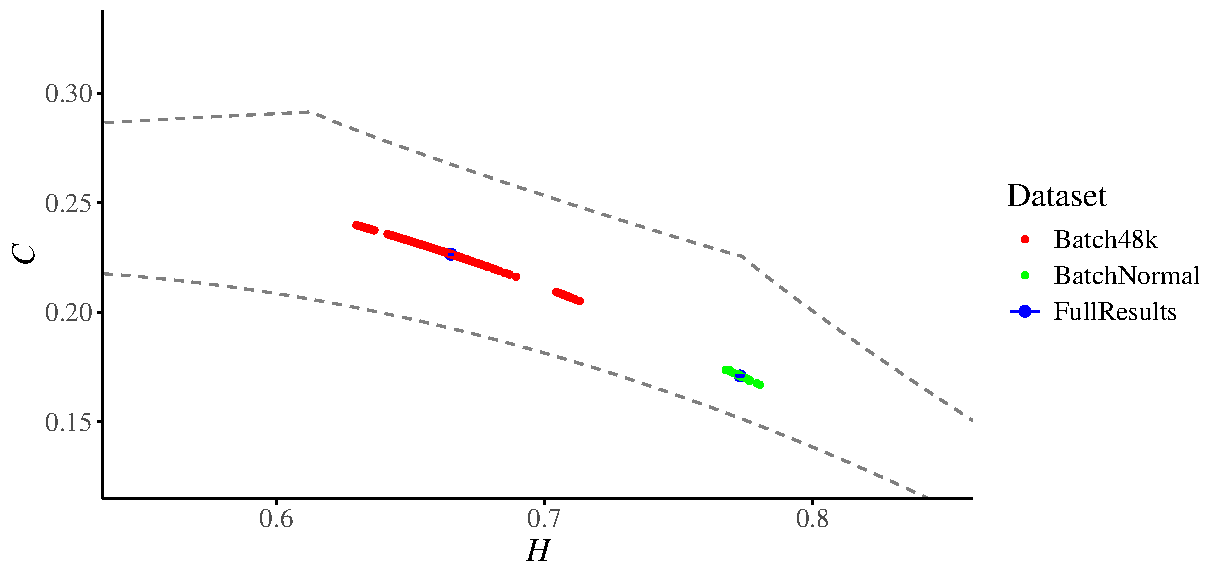
\includegraphics[width=0.6 \textwidth]{confidence_interval}
	%\caption{Entropy Complexity Plane}
	\label{fig:EntopyComplexity Plane}
\end{figure}
	\begin{itemize}
		\item Faulty machines form a distinct cluster in the entropy–complexity plane.
		\item Both overlapping and non-overlapping confidence intervals observed, indicating varying degrees of difference.
		\item Increasing embedding dimension is recommended for deeper analysis.
		\item The entropy–complexity plane highlights the separation between normal and faulty machinery.
	\end{itemize}
\end{frame}

\begin{frame}
	In addition to this we analyze the full data results for higher embedding dimension $D=6$.
		\begin{figure}[hbt]
		\centering
		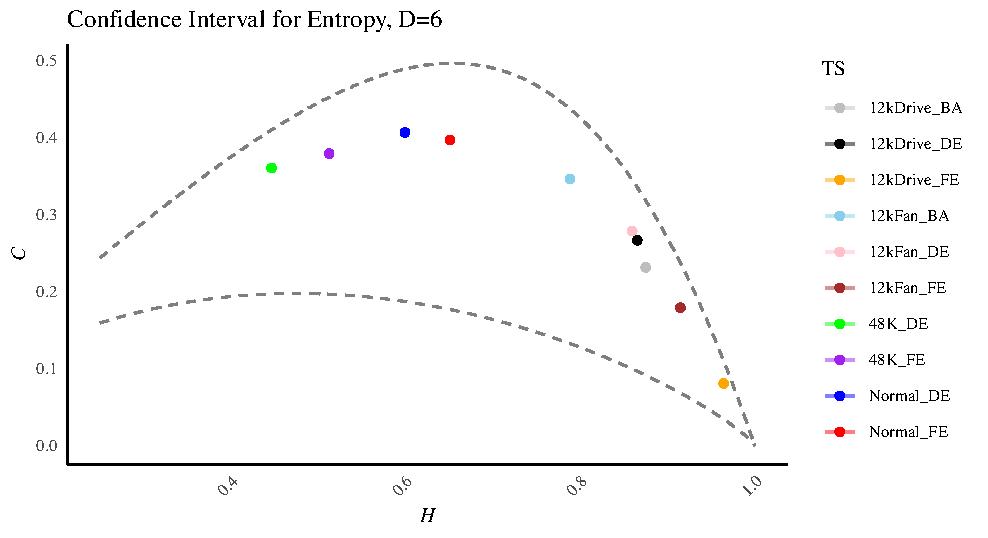
\includegraphics[width=0.8 \textwidth]{Confidence Interval}
		%\caption{Entropy Complexity Plane}
		\label{fig:EntopyComplexity Plane D=6}
	\end{figure}
\end{frame}


%---------------------%
\section{Future Plans}
%---------------------%

\begin{frame}{Future Plans}
    \begin{itemize}
        \item Define a data base of time series for clustering, i.e., finding similar time series.
        \item Extract all the features we know from their Bandt \& Pompe symbolization (Tsallis and Renyi entropies, Fisher information measure, complexities, and the available confidence intervals).
        \item Use those features for time series clustering
    \end{itemize}
\end{frame}

\begin{frame}[allowframebreaks]{References}
    \bibliographystyle{alpha}
    \bibliography{../BearingFaultDiagnosis}
    
\end{frame}
%Ending slides
\end{document}

Dávalos, A., Jabloun, M., Ravier, P., Buttelli, O., 2019. On the statistical properties of Multiscale Permutation Entropy: Characterization of the estimator’s variance, Entropy, 21, 5. doi: 10.3390/e21050450.
Please read it carefully, check the hypothesis and assumptions, and compare those results with ours. This would be an interesting contribution.
